\section{The cost of moving a deep structure}
\label{hrec:sec:actuation}
The gain calculation describes a response to a held broadcast. It does not say how an instruction moves through the physical structure. We therefore specify an actuator separately. Let \(z_t\in\mathbb R^L\), let \(e_i\) denote the coordinate basis vectors, and let \(S\) have ones on its first subdiagonal and zeros elsewhere. The base is coordinate one and the top is coordinate \(L\). For \(t=0,\ldots,H-1\), take
\begin{equation}
 \begin{gathered}
 z_{t+1}=A z_t+B v_t,\\
 A=aI+cS,\qquad B=g e_1.
 \end{gathered}
 \label{hrec:eq:chain}
\end{equation}
The persistence \(a\), transmission \(c\) and actuator gain \(g\) are specified properties of this model. A pure shift has \(a=0\). A persistent chain has \(a\ne0\), with \(a=1\) allowing local accumulation. The shift is not a chain of unit integrators.

An intervention task also needs an initial state \(z_0\), an integer horizon \(H\), a target and a cost metric. In chronological input order \(\bm v=(v_0,\ldots,v_{H-1})^\top\),
\begin{equation}
 \begin{gathered}
 z_H=A^H z_0+C_H\bm v,\\
 C_H=[A^{H-1}B,\ldots,AB,B].
 \end{gathered}
 \label{hrec:eq:chronological}
\end{equation}
A full terminal target \(z_*\) requires defect \(q=z_*-A^Hz_0\). A scalar top target \(e_L^\top z_H=\delta\) requires only
\(d_y=\delta-e_L^\top A^Hz_0\), leaving other terminal components free. Effort is
\begin{equation}
 J=\bm v^\top R_H\bm v,\qquad R_H\ \text{positive definite}.
 \label{hrec:eq:effort}
\end{equation}
For the uniform metric \(R_H=wI\), state units \(Z\), input units \(U\), \([g]=Z/U\) and \([w]=\text{effort}/U^2\). The reference \(E_0=w\delta^2/g^2\) has the chosen effort units. Those units are not necessarily joules. A terminal squared-input task does not become heat dissipation or sustained maintenance by renaming its cost.

Reachability comes before minimisation. Put \(\mathcal M=C_H\), \(b_q=q\) for a full target, or \(\mathcal M=e_L^\top C_H\), \(b_q=d_y\) for the top output. If \(b_q\notin\ran(\mathcal M)\), the exact task is infeasible and its extended minimum is \(+\infty\). If it is reachable, whitening by \(R_H^{1/2}\) gives the unique optimum
\begin{align}
 \bm v_*&=R_H^{-1}\mathcal M^\top
       (\mathcal M R_H^{-1}\mathcal M^\top)^+b_q,\nonumber\\
 J_{\min}&=b_q^\top(\mathcal M R_H^{-1}\mathcal M^\top)^+b_q.
 \label{hrec:eq:min-effort}
\end{align}
The superscript \(+\) denotes the Moore--Penrose pseudoinverse. It is not a substitute for the reachability condition. An unreachable top direction can have zero pseudoinverse quadratic, which is not zero effort to reach it.

The chain's impulse response follows from the commuting terms \(aI\) and \(cS\):
\begin{equation}
 A^jB=g\sum_{i=0}^{\min(j,L-1)}
       \binom ji a^{j-i}c^i e_{i+1}.
 \label{hrec:eq:impulse}
\end{equation}
For \(gc\ne0\), the first \(\min(H,L)\) power columns are triangular with nonzero successive diagonal entries \(gc^j\), so \(\operatorname{rank}C_H=\min(H,L)\). Starting from zero, a nonzero top target is unreachable for \(H<L\), however large the input budget.

For a pure shift, only \(v_{H-L}\) can reach the top at time \(H\). When \(H\ge L\), choosing \(v_{H-L}=\delta/(gc^{L-1})\) and all other inputs zero gives
\begin{equation}
 J_{\rm top}=E_0c^{-2(L-1)}.
 \label{hrec:eq:shift-cost}
\end{equation}
It also makes all lower terminal components zero. Thus the scalar top and full pure-apex targets \(z_*=\delta e_L\) have identical cost in this special case. Extra time beyond \(L\) gives no further reduction, because the shift's finite-horizon Gramian has already saturated.

Persistence changes both conclusions. Consider \(L=2,a=1,c=1/2,g=w=1,z_0=0\), with top target one. At \(H=2\), the chronological scalar-optimal input \((2,0)\) leaves \(z_2=(2,1)\), at cost four. To finish instead at the pure apex \((0,1)\), the input must be \((2,-2)\), at cost eight. The extra input cancels the lower terminal component. The scalar solution is cheaper because it solves a less restrictive task, not because it finds a better solution to the same full-state problem. At \(H=3\), the scalar control is \((0.8,0.4,0)\), with cost \(4/5\), whereas \((1,0,-1)\) reaches the pure apex with cost two.

\begin{figure}[t]
 \centering
 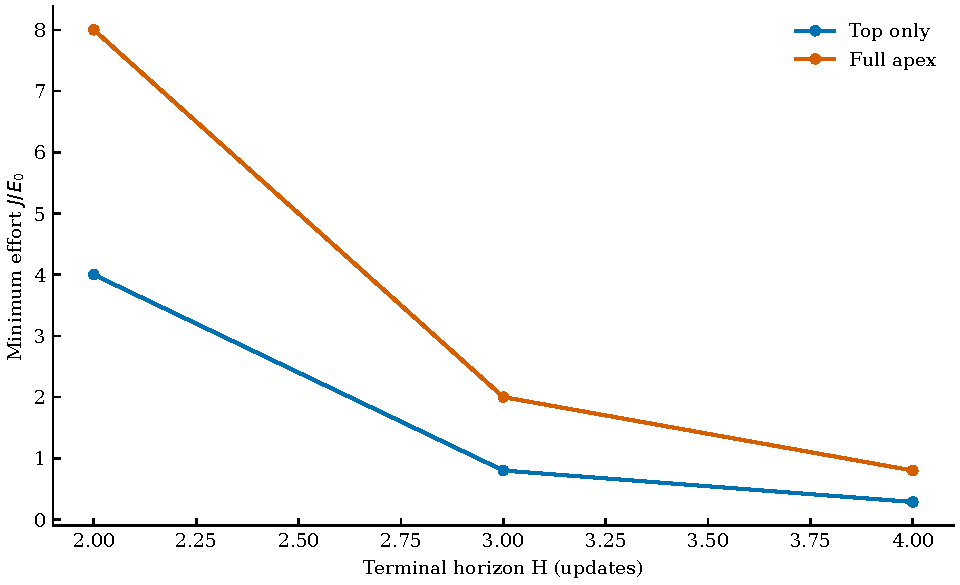
\includegraphics[width=\columnwidth]{figures/generated/persistent-terminal-effort-paper.pdf}
 \caption{Time helps according to the terminal task. Retained numerical optima for the two-state persistent chain \(a=1,c=1/2,g=w=1,z_0=0\). The top-only target is \(z_2(H)=1\). The full-apex target additionally requires \(z_1(H)=0\). Only the declared horizons \(H=2,3,4\) are plotted, with lines joining these samples as visual guides. At \(H=1\), both nonzero top tasks are unreachable, not zero-cost. The normalisation is \(E_0=1\) in illustrative squared-input units. No calibrated physical energy or uncertainty model is implied.}
 \label{hrec:fig:effort}
\end{figure}

The horizon theorem has an equally definite scope. For zero initial state, a fixed terminal target and uniform positive metric, minimum full-state effort is nonincreasing as \(H\) grows. With \(W_H=C_HC_H^\top\), full rank holds for \(H\ge L\). Writing \(v_H=A^HB\), Sherman--Morrison gives
\begin{equation}
 J_H-J_{H+1}
 =\frac{w(q^\top W_H^{-1}v_H)^2}
        {1+v_H^\top W_H^{-1}v_H}\ge0.
 \label{hrec:eq:horizon}
\end{equation}
Improvement is strict only when the numerator is nonzero. In the same two-state chain, the \emph{different} full target \(q=(6,1)^\top\) has effort 20 at both \(H=2\) and \(H=3\). For top-only targets, every extra impulse-response term is positive when \(a\ne0\), so effort decreases strictly once \(H\ge L\). Appendix~\ref{hrec:app:control} proves these claims and covers singular reachable cases.

We can now combine the two constructions without conflating their coefficients. Let \(\mathcal A(N)\) be the admitted architecture set, and assign to each architecture its actual controller gain and its specified actuation model. Then
\begin{equation}
 \mathcal F(N)=\left\{\mathcal T\in\mathcal A(N):
 \begin{array}{l}
 0<K_{\mathcal T}<K_c,\\
 b_q\in\ran(\mathcal M_{\mathcal T,H}),\\
 J_{\min}(\mathcal T,H)\le E_{\max}
 \end{array}\right\}.
 \label{hrec:eq:feasibility}
\end{equation}
The inequality refers to the corresponding controller's local criterion. It does not certify a global attractor. Static gain attenuation \(d\) and actuator transmission \(c\) enter different calculations. A relation such as \(d=c^2\) would be an additional coupling hypothesis, not a consequence of reversing a many-to-one majority map.

A simple depth window is a conditional specialisation of Eq.~\eqref{hrec:eq:feasibility}. For the zero-initial-state shift task, \(0<c<1\), \(H\ge1\), and \(E_{\max}/E_0\ge1\),
\begin{equation}
 L\le L_{\rm cap}=\min\left\{H,\,
 1+\left\lfloor\frac{\log(E_{\max}/E_0)}{\log(c^{-2})}\right\rfloor\right\}.
 \label{hrec:eq:budget-cap}
\end{equation}
If all integer depths from one to \(L_{\rm cap}\) are admitted and Eq.~\eqref{hrec:eq:depth-law} is valid, feasibility reduces to \(L_{\min}(N)\le L_{\rm cap}\). Its size bound is the strict supremum
\begin{equation}
 N<N_{\rm sup}=N_{\rm ref}(K_c/K_{\rm ref})^{1/p}
 d^{-(L_{\rm cap}-1)/p}.
 \label{hrec:eq:conditional-size}
\end{equation}
The budget allows equality, whereas stability does not. Actual product-tree sizes must still be intersected with their admitted set. Persistent chains generally require the task-specific Gramian rather than this shift-only ceiling.

